\section{Índices de governo eletrônico}

Existem 4 tipos de índices de governo eletrônico, segundo \cite{martinez2022egovernment}: EDGI da ONU, GTMI do Banco Mundial, DESI da Comissão Europeia da União Europeia e DGI da OECD.

A não escolha do DESI foi motivada pela explicação de \cite{desi_2022} de como ó índice funciona. De acordo com \cite{desi_2022}, como o DESI é administrado pela Comissão Europeia da UE, ele foca no análise individual de cada Estado membro da UE para que eles possam identificar áreas que precisam de ações prioritárias. Além disso, os relatórios do DESI possuem capítulos temáticos que providenciam analises a nível supranacional em áreas de áreas chave de política digital.

\subsection{EGDI}

O EGDI apresenta o estado de desenvolvimento de governo eletrônico dos Estados membro da ONU. O índice incorpora as características de acesso, tais como níveis de infraestrutura e educacional para mostrar como um país está usando as tecnologias de informação para promover acesso e inclusão do seu povo \cite{ONU_egdi}.

\cite{ONU_egdi} afirma que o EGDI é uma mensuração composta formada por 3 importantes dimensões do governo eletrônico: provisão de serviços online, conectividade de telecomunicação e capacidade humana.

Os componentes do EGDI são:

\begin{figure}[H]
	\centering
	\caption{Componentes do EGDI}
	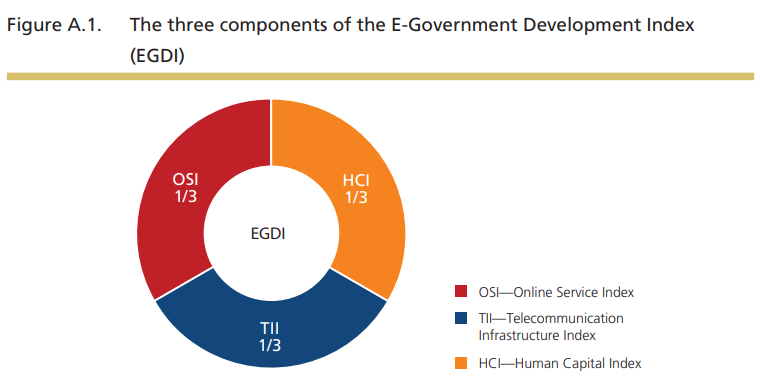
\includegraphics[width=1\linewidth]{figuras/egdi/egdi_componentes.png}
	\label{fig:egdi_componentes}
	\footnotesize{Fonte: \cite{ONU_egdi_methodology}}
\end{figure}

A figura \ref{fig:boxplot_egov_global} contém um diagrama de caixa que representa o EGDI global.

\begin{figure}[H]
	\centering
	\caption{E-Government Development Index global em 2024}
	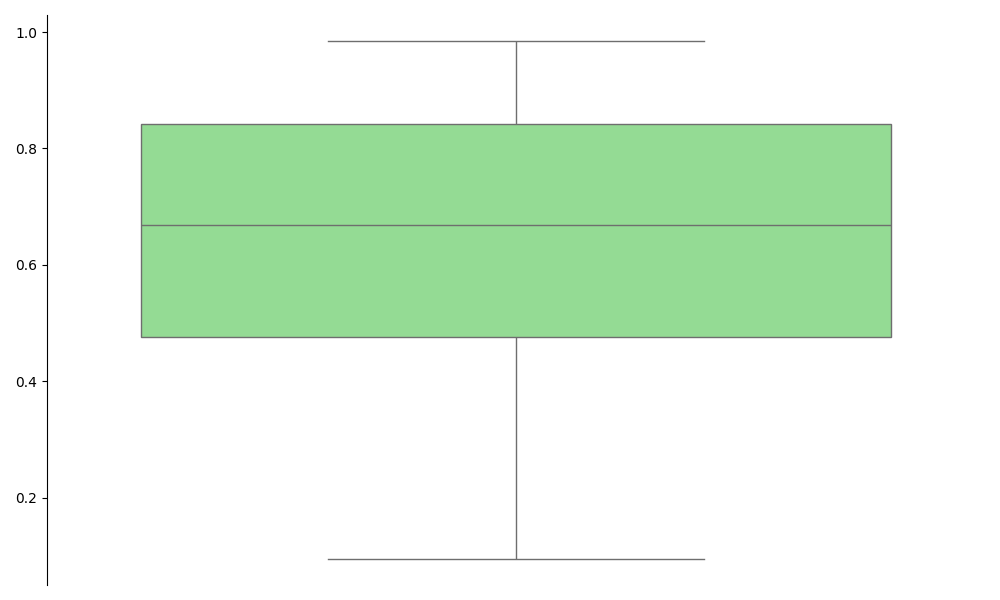
\includegraphics[width=1\linewidth]{figuras/egdi/boxplot_egov_global.png}
	\label{fig:boxplot_egov_global}
	\footnotesize{Fonte: baseado em \cite{ONU_edgi_mapa}.}
\end{figure}

A linha central na caixa indica que a mediana do índice é de aproximadamente 0.65. A caixa em si, que representa os 50\% centrais dos dados, se estende de cerca de 0.48 a 0.83, mostrando a variação dos índices na maioria dos países. As linhas verticais, conhecidas como "bigodes", demonstram a amplitude total dos dados, que vai de aproximadamente 0.1 a quase 1.0. A distribuição do índice parece ser relativamente simétrica, sem um viés perceptível para valores mais altos ou mais baixos, e o gráfico não identifica a presença de valores discrepantes (outliers) extremos.

\subsubsection{E-Participation Index}
\label{epart}

\cite{ONU_egdi} argumenta que o \textbf{E-Participation Index} deriva do EGDI como índice suplementar ao relatório \textbf{E-Government Survey}. Os componentes do índice são: \textbf{E-information}, \textbf{E-consultation} e \textbf{E-decision-making}. 

\textbf{E-information} fala sobre a facilitação da participação dos cidadãos via informações públicas e acesso a informação sem necessidade de pedido ou sob demanda. \textbf{E-consultation} diz respeito ao engajamento dos cidadãos em contribuições e deliberações sobre políticas publicas e serviços públicos. \textbf{E-decision-making} engloba o empoderamento dos cidadãos via a opção de coparticipação na elaboração de políticas e coprodução de componentes de serviços e entrega de modalidades.

\cite{ONU_egdi} esclarece que o \textbf{E-Participation Index} de um país reflete os mecanismos do índice que são empregados pelo governo quando se faz comparações com todos outros países. 

O propósito dessa medição não é prescrever qualquer prática especificam, no entanto oferece perspectivas de como países diferentes estão usando ferramentas online para promover interação entre o governo e seu povo, bem como, entre as pessoas para benefícios de todos.

A figura \ref{fig:boxplot_epart_global} contém um diagrama de caixa que representa o \textbf{E-Participation Index} global.

\begin{figure}[H]
	\centering
	\caption{E-Participation Index global}
	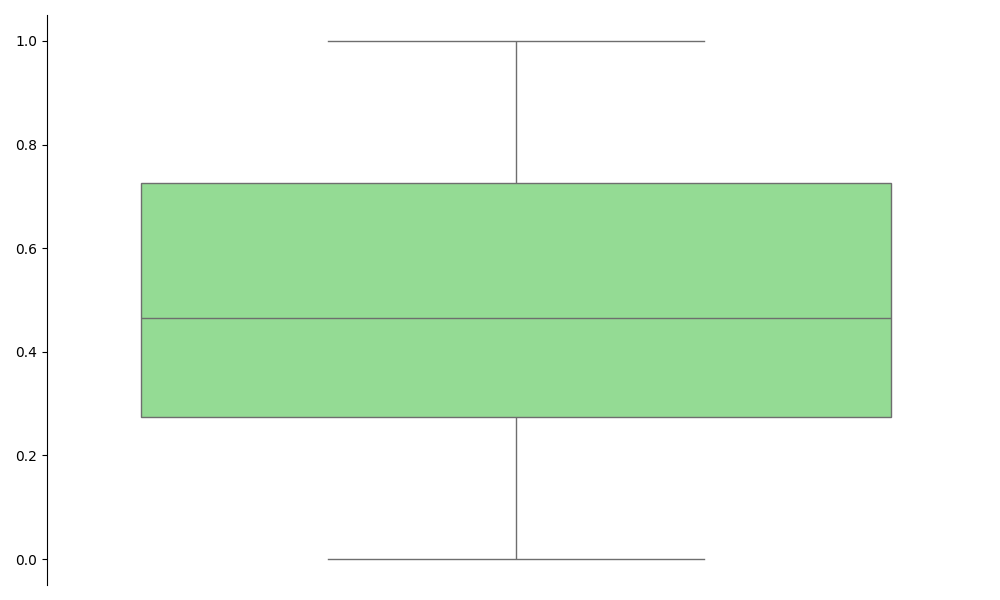
\includegraphics[width=1\linewidth]{figuras/egdi/boxplot_epart_global.png}
	\label{fig:boxplot_epart_global}
	\footnotesize{Fonte: baseado em \cite{ONU_edgi_mapa}.}
\end{figure}

A figura \ref{fig:boxplot_epart_global} revela que a mediana do índice é de aproximadamente 0.47, indicando que metade dos países avaliados se encontra acima desse valor. A caixa do gráfico abrange o intervalo entre 0.28 e 0.72, onde estão concentrados 50\% dos países. A amplitude total dos índices é considerável, variando de 0.0 a 1.0. A distribuição se apresenta como relativamente simétrica, sem uma concentração significativa de países nas extremidades dos dados, e não há indícios de valores discrepantes (outliers).

\subsubsection{Online Service Index}
\label{osi}

A figura \ref{fig:boxplot_osi_global} contém um diagrama de caixa que representa o \textbf{E-Participation Index} global.

\begin{figure}[H]
	\centering
	\caption{Online Service Index global}
	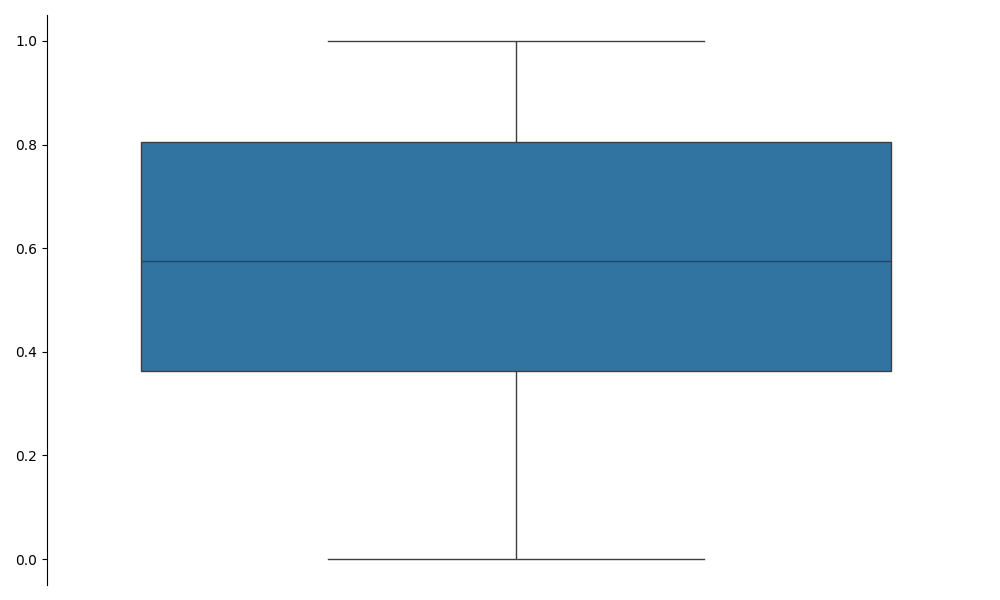
\includegraphics[width=1\linewidth]{figuras/egdi/boxplot_osi_global.png}
	\label{fig:boxplot_osi_global}
	\footnotesize{Fonte: baseado em \cite{ONU_edgi_mapa}.}
\end{figure}

A figura \ref{fig:boxplot_osi_global} revela que a mediana do índice de serviços online é de aproximadamente 0.58. A caixa principal do gráfico indica que 50\% dos países têm índices que variam entre 0.38 e 0.81. A amplitude total dos dados é vasta, indo de 0.0 a 1.0, o que demonstra uma grande disparidade nos níveis de serviços online oferecidos globalmente. A distribuição dos dados é relativamente simétrica e, assim como nos gráficos anteriores, não há outliers visíveis.

\subsubsection{Human Capital Index}
\label{hci}

\cite{ONU_egdi_methodology} afirma que \textbf{Human Capital Index} tem 4 indicadores: taxa bruta de matrícula, letramento adulto, anos de escolarização esperados e média de anos de escolaridade. 

A taxa bruta de matrícula é medida como a combinação entre a taxa de matrícula nas educações primárias, secundários e terciárias. Letramento adulto é medido como o percentual de pessoas com pelos menos 15 anos de idade que entendem e sabem ler e escrever um frase curta simples na sua vida padrão.

Os anos de escolarização esperados é o número total de anos de escolarização que crianças de certa idade podem esperar ter no futuro, presumindo que a probabilidade de a criança de qualquer idade estiver na escola correspondendo à idade da taxa de matrícula atual.

A média de anos de escolaridade fornece o número médio de anos de educação concluídos pela população adulta de um país (25 anos ou mais), excluindo os anos gastos repetindo séries. 

A figura \ref{fig:boxplot_hci_global} contém um diagrama de caixa que representa o \textbf{E-Participation Index} global.

\begin{figure}[H]
	\centering
	\caption{Human Capital Index global}
	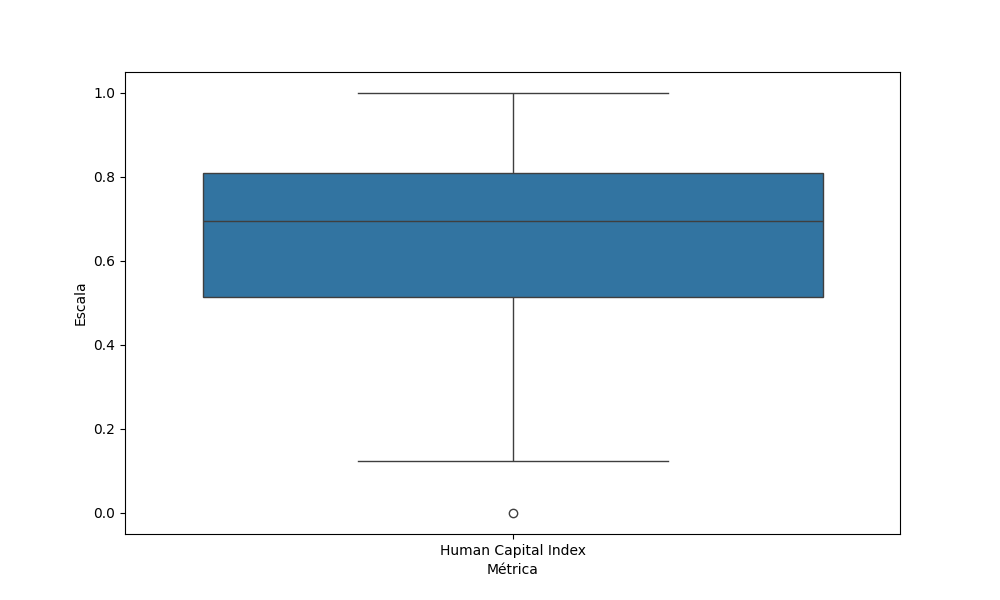
\includegraphics[width=1\linewidth]{figuras/egdi/boxplot_hci_global.png}
	\label{fig:boxplot_hci_global}
	\footnotesize{Fonte: baseado em \cite{ONU_edgi_mapa}.}
\end{figure}

A figura \ref{fig:boxplot_hci_global} mostra que a mediana do índice de capital humano é de aproximadamente 0.70. A caixa principal, que concentra os 50\% centrais dos dados, indica que a maioria dos países tem um índice que varia entre 0.52 e 0.81. A amplitude dos dados é ampla, indo de cerca de 0.13 a 1.0. A distribuição se apresenta como relativamente simétrica, e, diferentemente dos gráficos anteriores, este diagrama aponta a existência de um outlier, um valor discrepante isolado, localizado próximo ao zero no eixo vertical, indicando um país com um índice de capital humano excepcionalmente baixo em comparação com os demais.

\subsubsection{Telecommunication Infrastructure Index}
\label{tii}

\cite{ONU_egdi_methodology} afirma que o \textbf{Telecommunication Infrastructure Index} tem 5 componentes: usuário de internet, assinatura de banda larga fixa, assinatura de banda larga sem fio, assinatura de telefone fixo e assinatura de dados móveis.

A figura \ref{fig:boxplot_tci_global} contém um diagrama de caixa que representa o \textbf{E-Participation Index} global.

\begin{figure}[H]
	\centering
	\caption{Telecommunication Infrastructure Index global}
	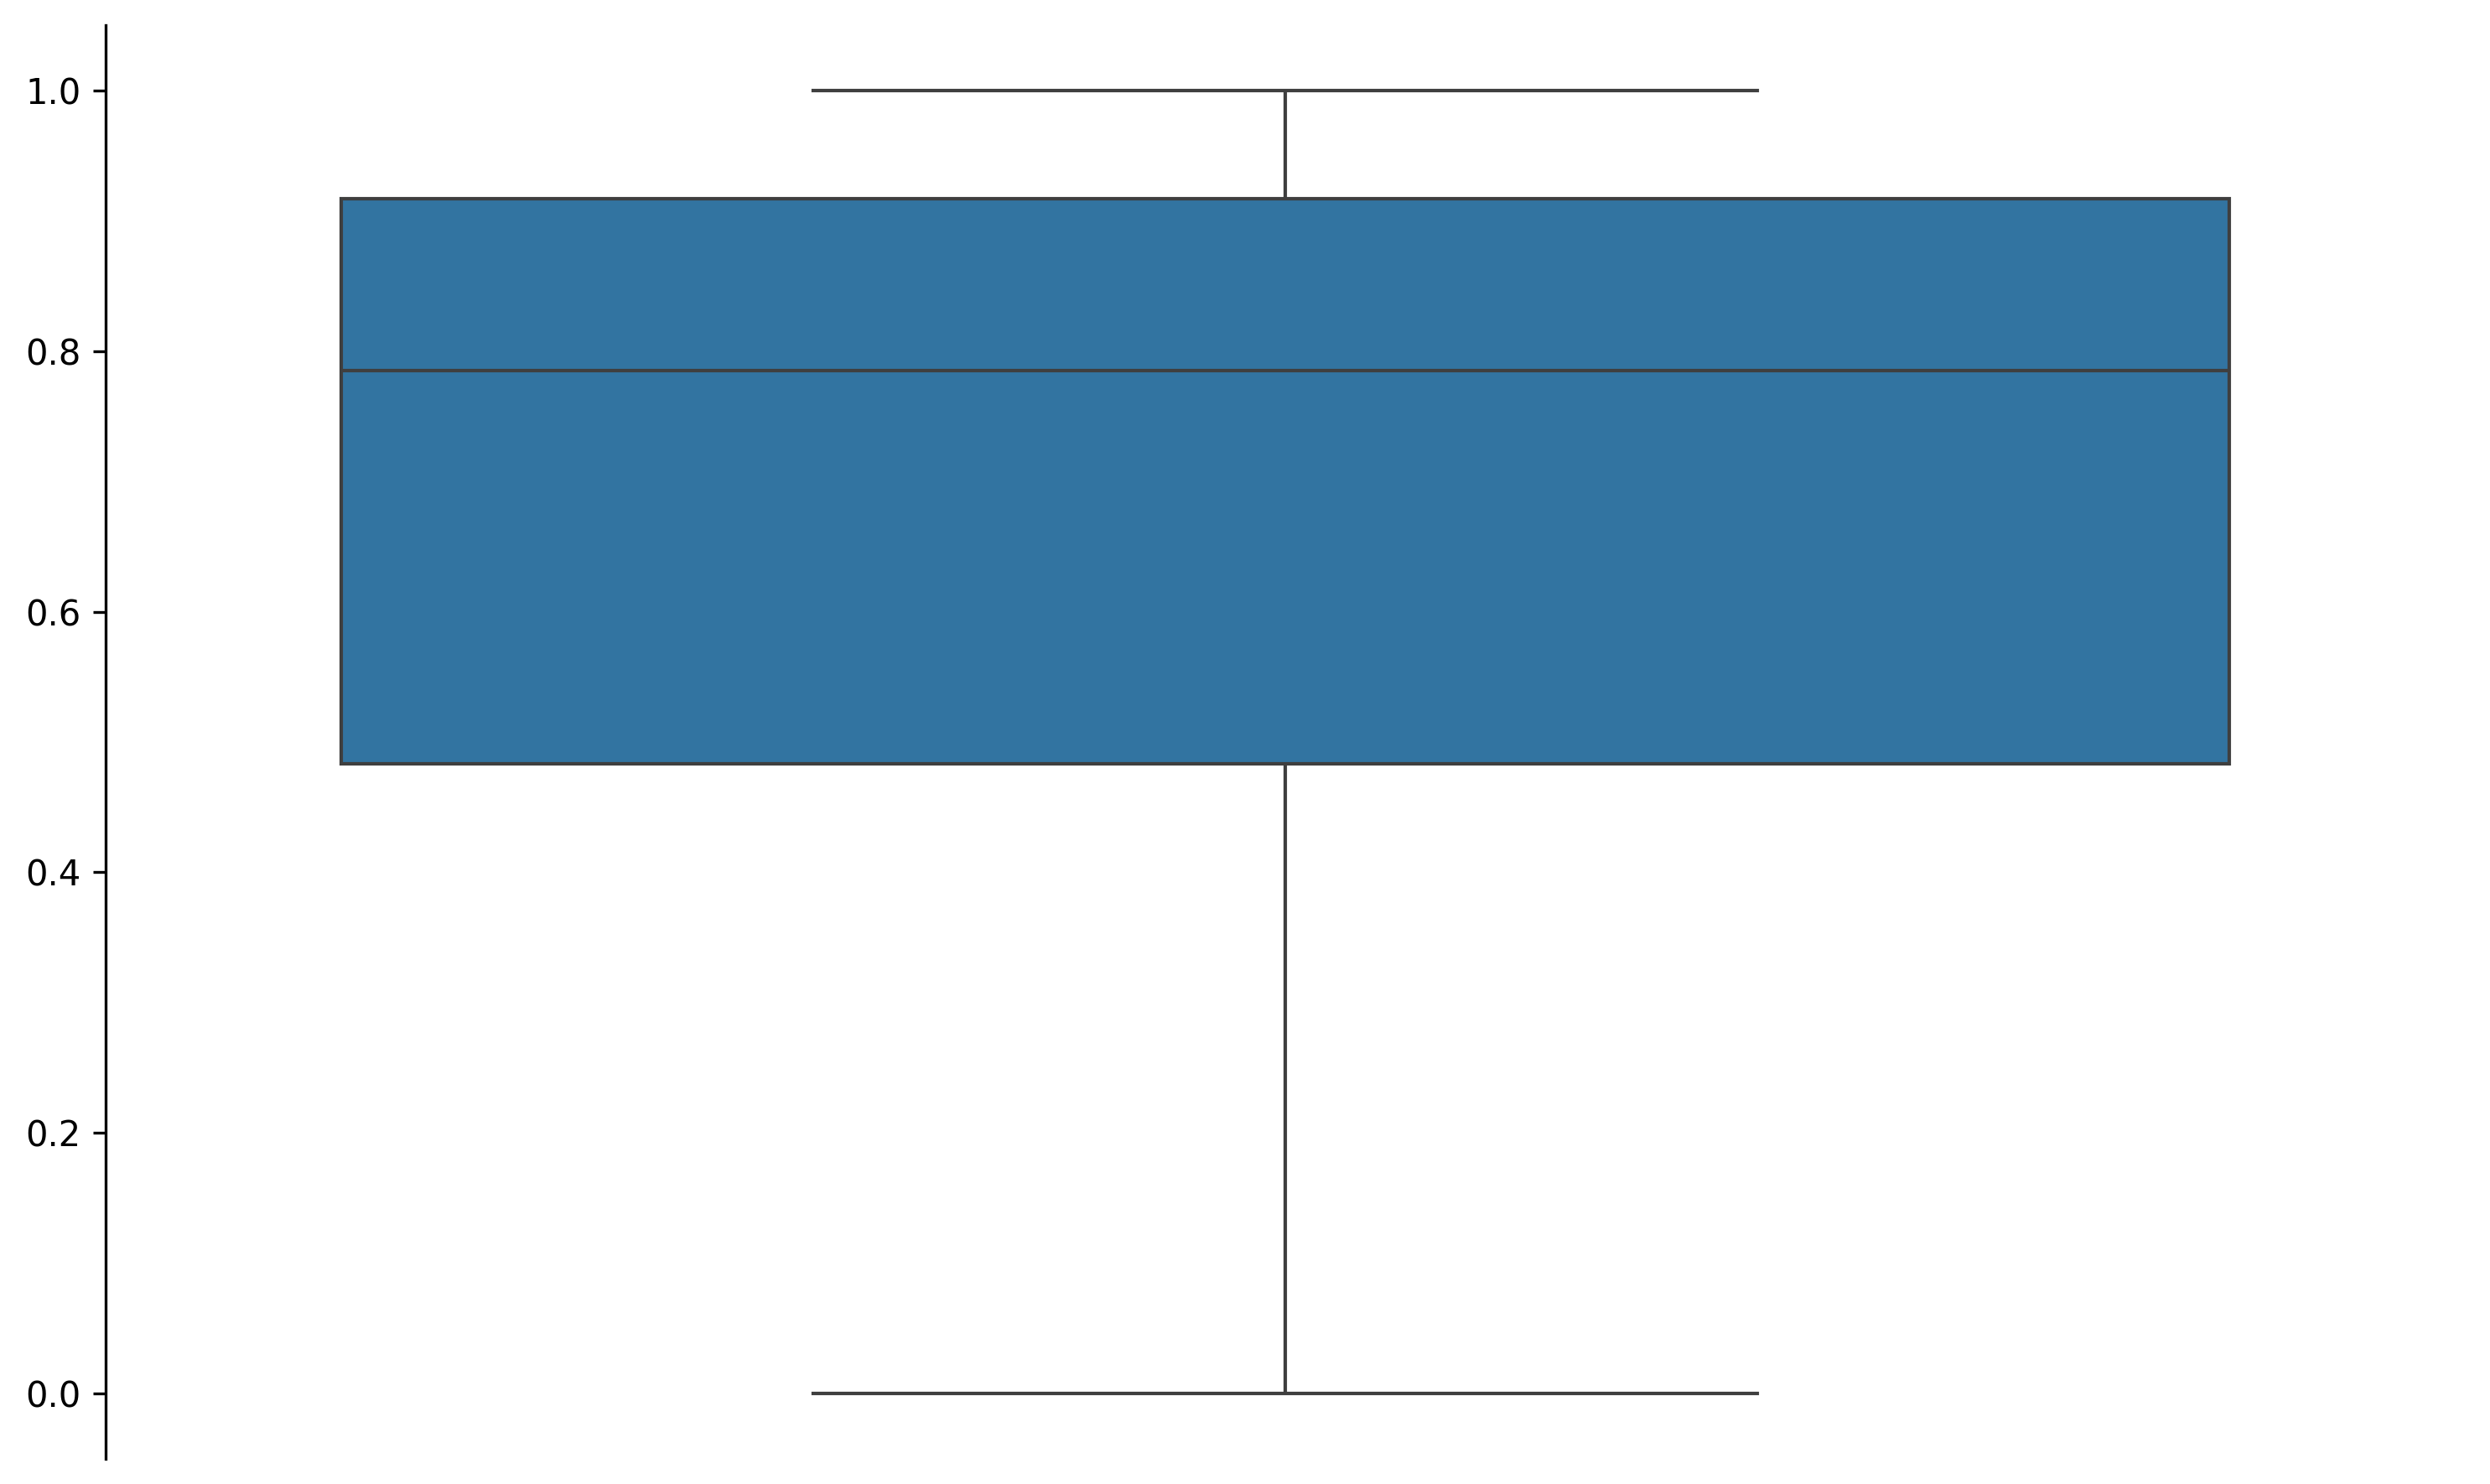
\includegraphics[width=1\linewidth]{figuras/egdi/boxplot_tci_global.png}
	\label{fig:boxplot_tci_global}
	\footnotesize{Fonte: baseado em \cite{ONU_edgi_mapa}.}
\end{figure}

A figura \ref{fig:boxplot_tci_global} mostra que a mediana do índice de infraestrutura de telecomunicações está em cerca de 0.80, indicando que metade dos países possui um índice superior a esse valor. A caixa do gráfico, que representa os 50\% centrais dos dados, abrange o intervalo entre aproximadamente 0.50 e 0.90. A amplitude total dos dados varia de 0.0 a 1.0. A distribuição dos dados é relativamente simétrica e, assim como na maioria dos gráficos anteriores, não há outliers visíveis.

\subsubsection{EGDI do Brasil}

A figura \ref{fig:lineplot_egdi_brasil} mostra evolução do EGDI do Brasil desde 2003-2005 e 2008-2024 (bianualmente)

\begin{figure}[H]
	\centering
	\caption{Evolução do EGDI do Brasil}
	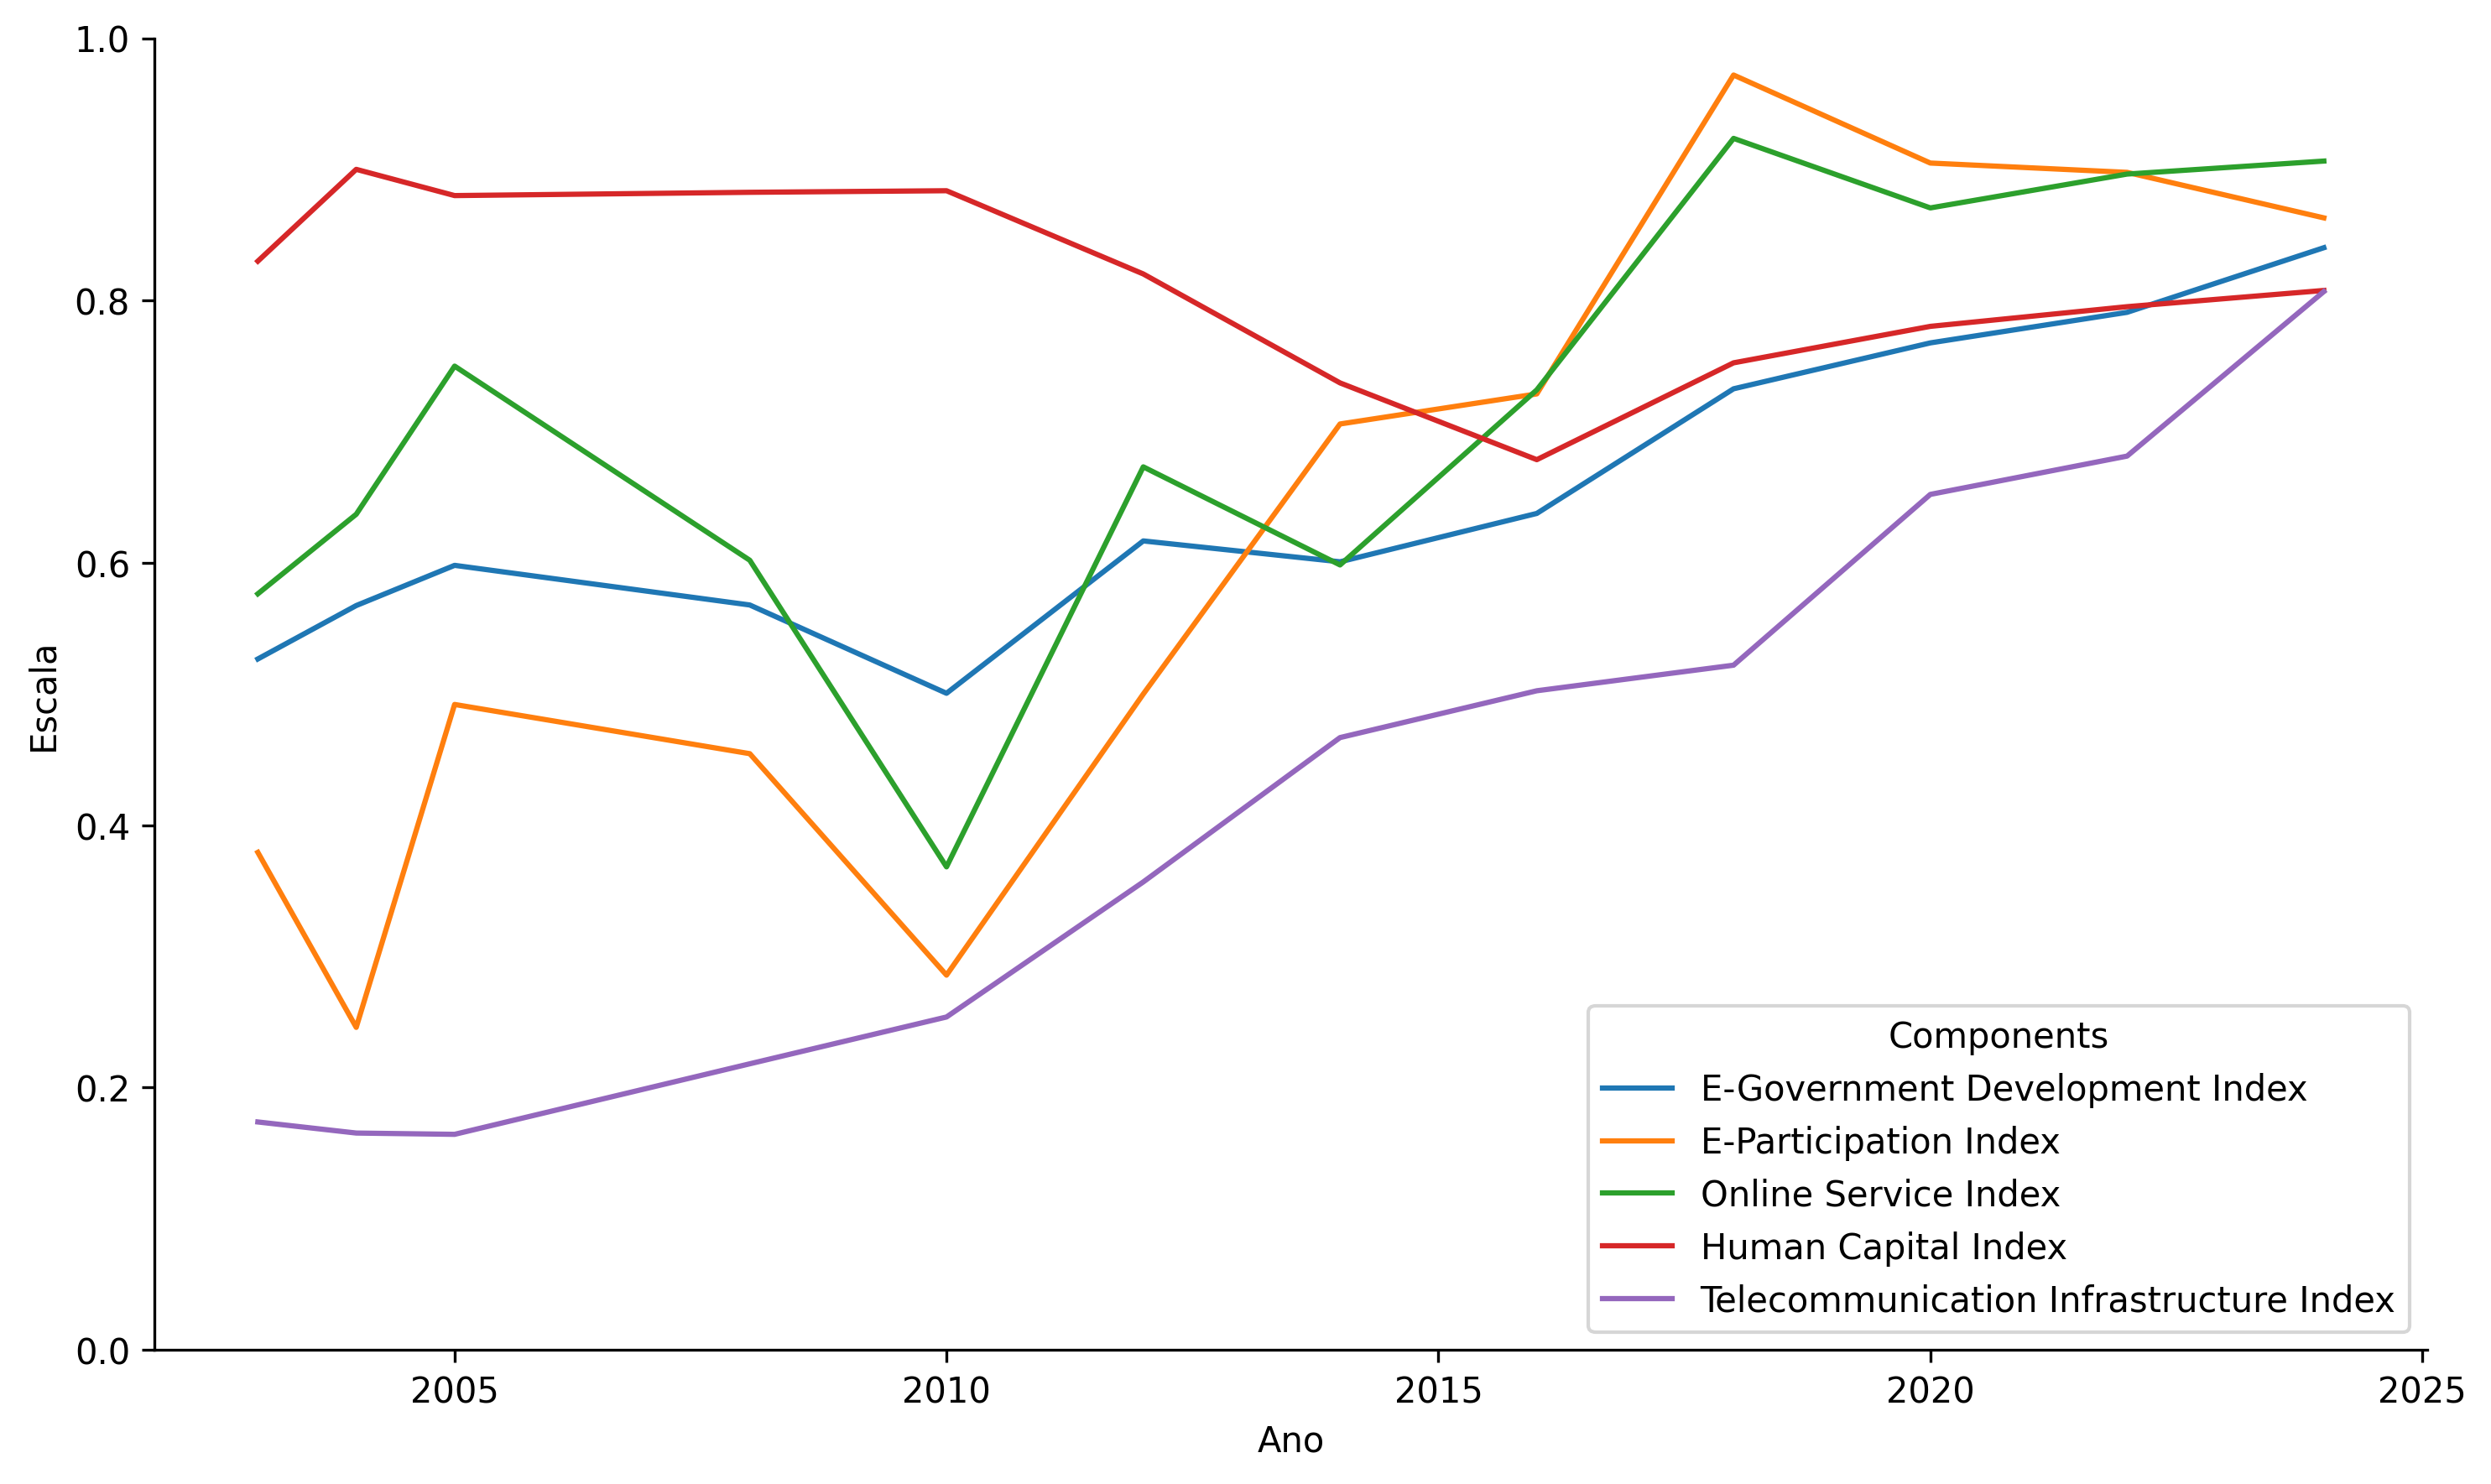
\includegraphics[width=1\linewidth]{figuras/egdi/lineplot_egdi_brasil.png}
	\label{fig:lineplot_egdi_brasil}
	\footnotesize{Fonte: baseado em \cite{ONU_edgi_mapa}.}
\end{figure}

\begin{figure}[H]
	\centering
	\caption{EGDI do Brasil}
	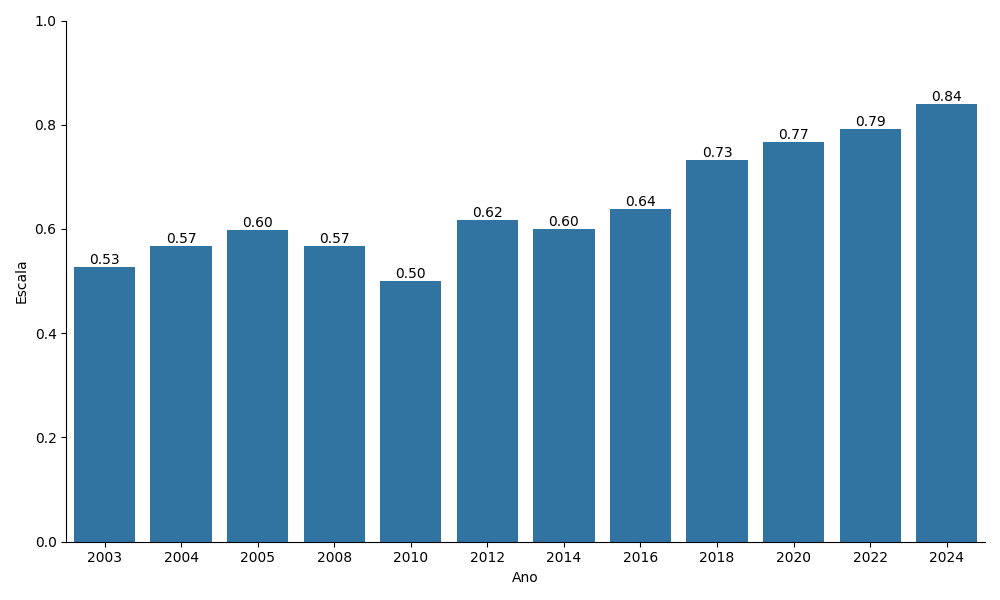
\includegraphics[width=1\linewidth]{figuras/egdi/egdi_brasil_egov.png}
	\label{fig:egdi_brasil_egov}
	\footnotesize{Fonte: baseado em \cite{ONU_edgi_mapa}.}
\end{figure}

\paragraph{E-Participation Index}

\begin{figure}[H]
	\centering
	\caption{EGDI do Brasil: E-Participation Index}
	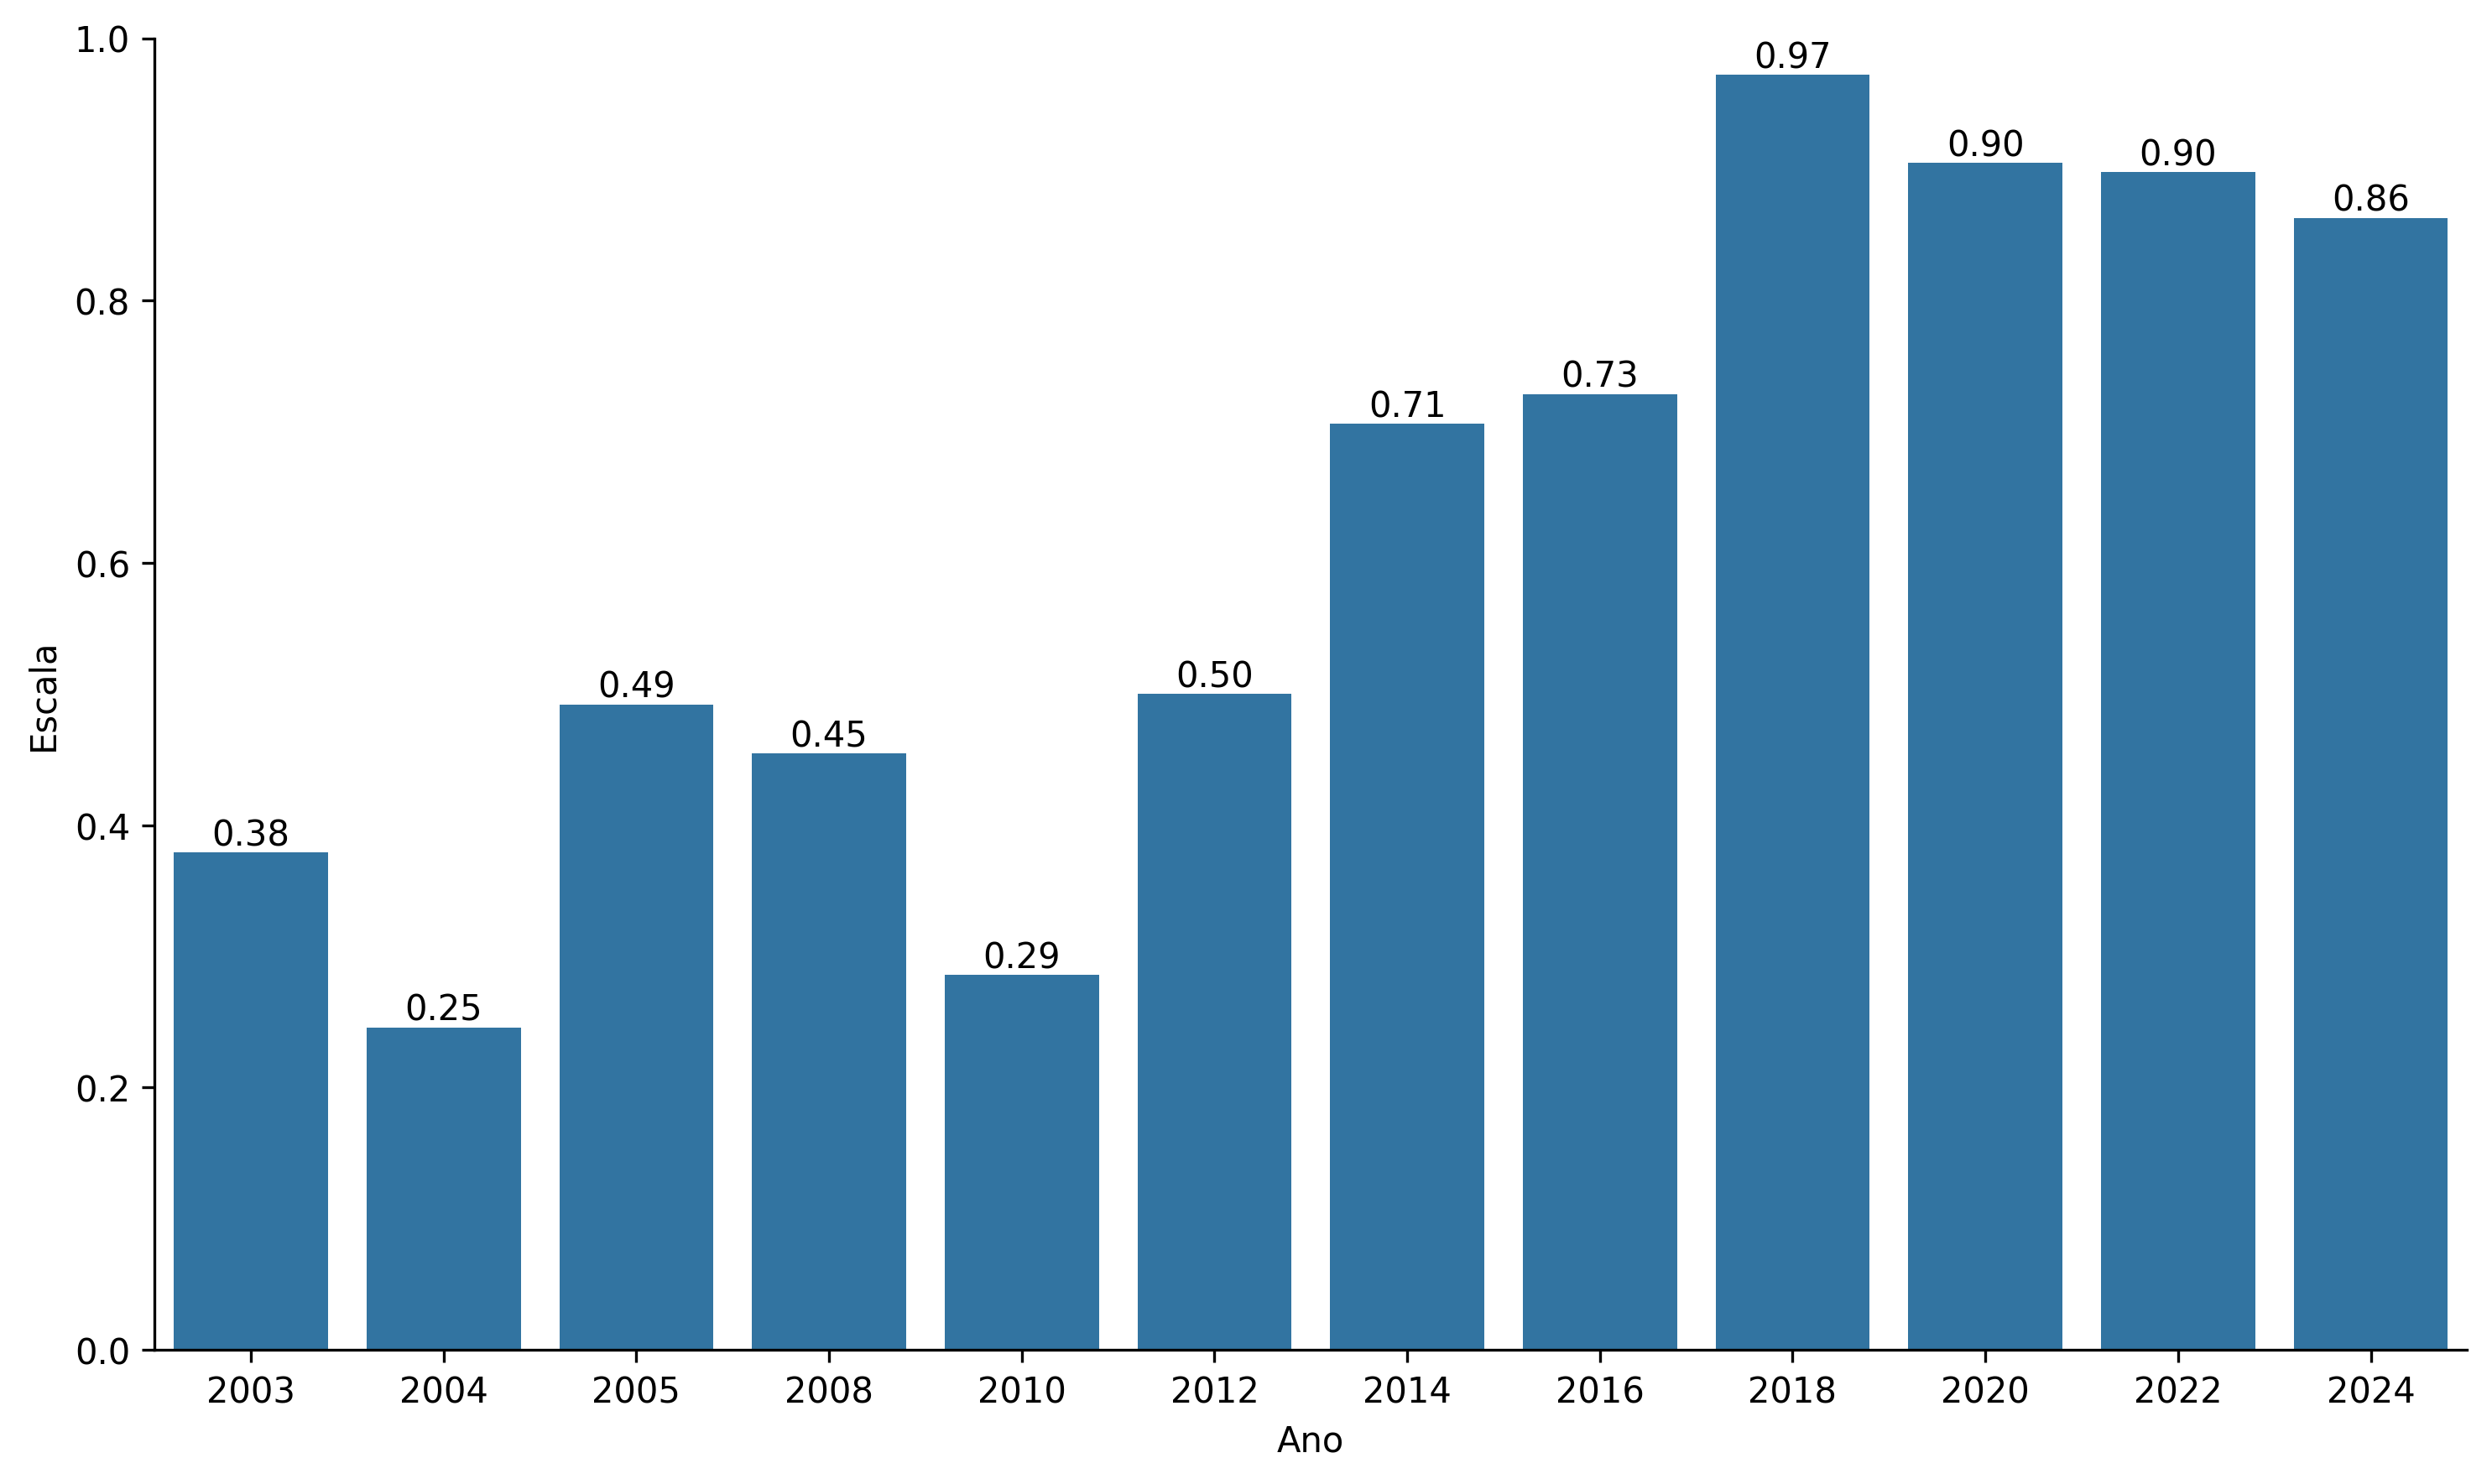
\includegraphics[width=1\linewidth]{figuras/egdi/egdi_brasil_epart.png}
	\label{fig:egdi_brasil_epart}
	\footnotesize{Fonte: baseado em \cite{ONU_edgi_mapa}.}
\end{figure}

\paragraph{Online Service Index}

\begin{figure}[H]
	\centering
	\caption{EGDI do Brasil: Online Service Index}
	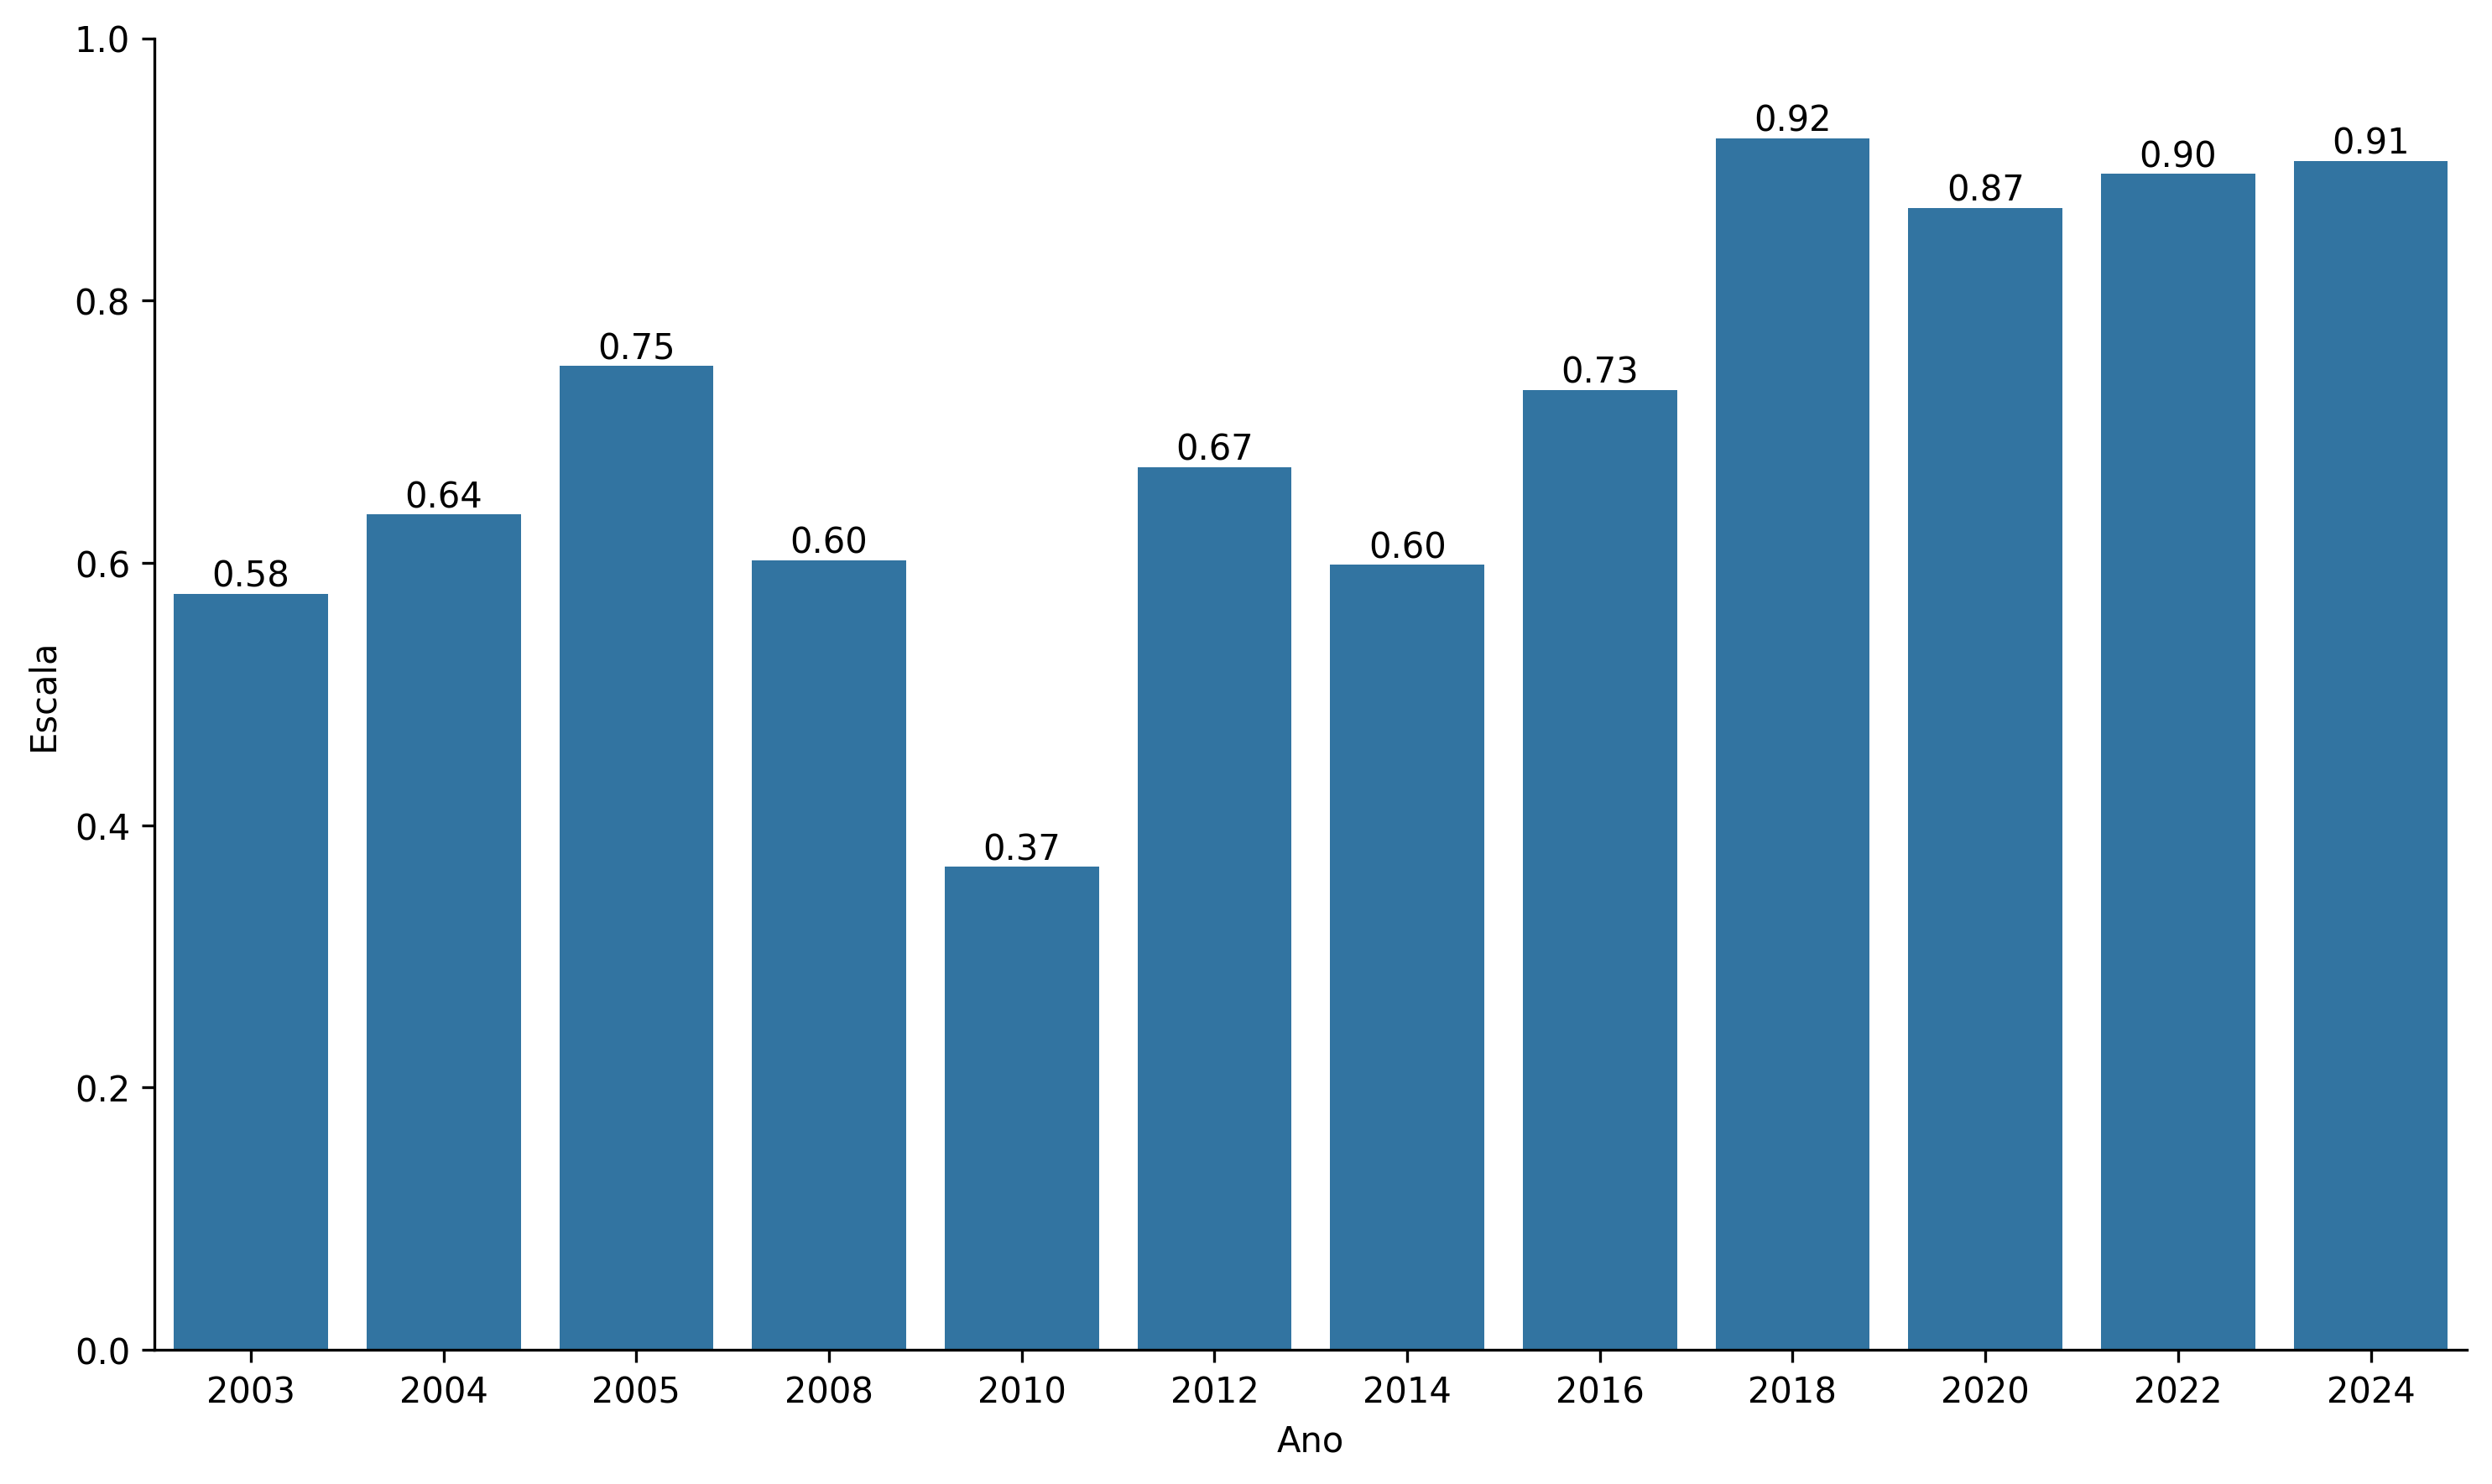
\includegraphics[width=1\linewidth]{figuras/egdi/egdi_brasil_osi.png}
	\label{fig:egdi_brasil_osi}
	\footnotesize{Fonte: baseado em \cite{ONU_edgi_mapa}.}
\end{figure}

\paragraph{Human Capital Indexx}

\begin{figure}[H]
	\centering
	\caption{EGDI do Brasil: Human Capital Index}
	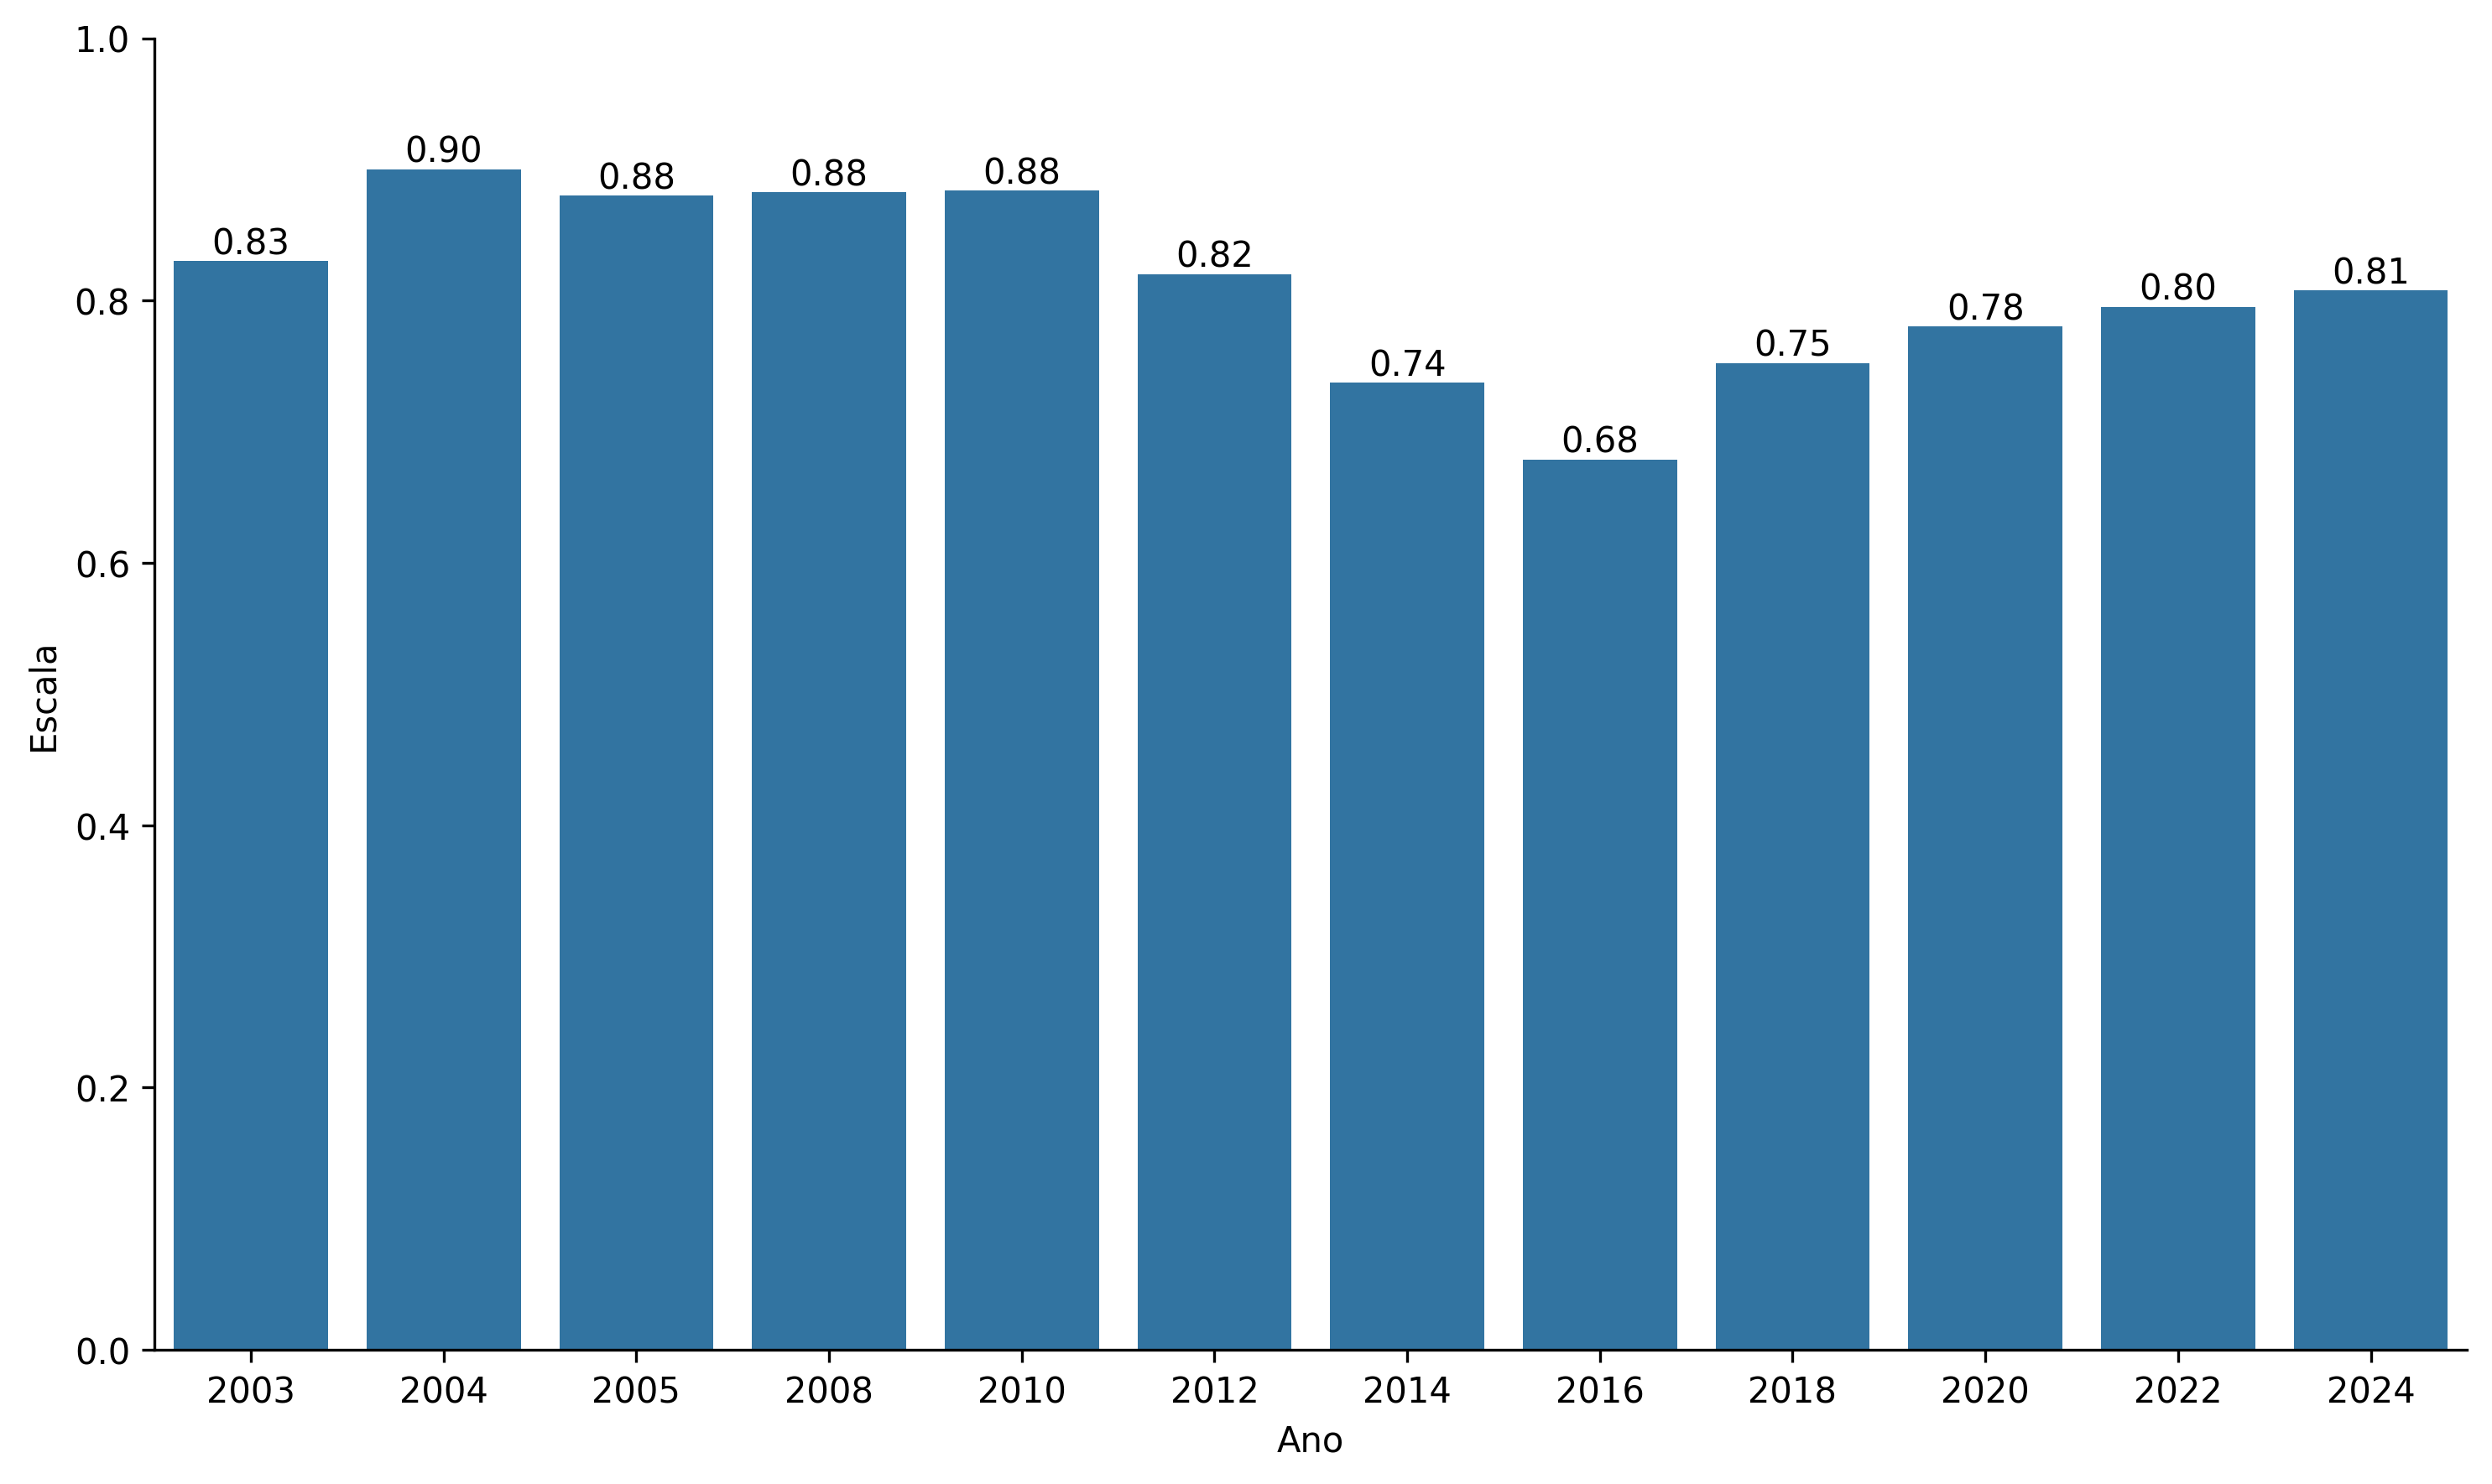
\includegraphics[width=1\linewidth]{figuras/egdi/egdi_brasil_hci.png}
	\label{fig:egdi_brasil_hci}
	\footnotesize{Fonte: baseado em \cite{ONU_edgi_mapa}.}
\end{figure}

\paragraph{Telecommunication Infrastructure Index}

\begin{figure}[H]
	\centering
	\caption{EGDI do Brasil: Telecommunication Infrastructure Index}
	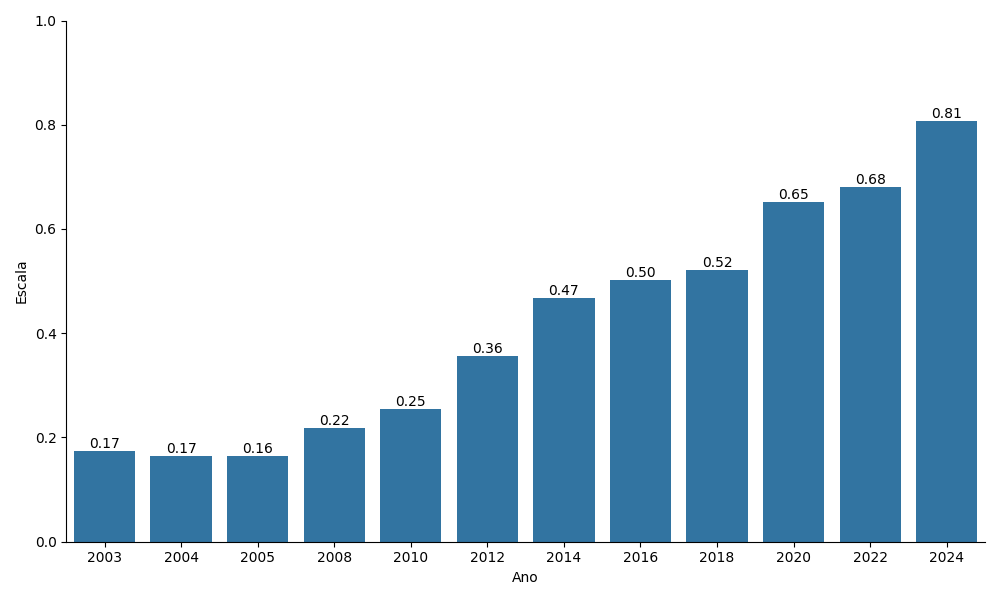
\includegraphics[width=1\linewidth]{figuras/egdi/egdi_brasil_tsi.png}
	\label{fig:egdi_brasil_tsi}
	\footnotesize{Fonte: baseado em \cite{ONU_edgi_mapa}.}
\end{figure}

\subsubsection{Coeficiente de correlação de Spearman: EGDI, E-Participation, índice de democracia eleitoral e PIB \textit{per capital}}

Ao analisar os dados do \href{https://publicadministration.un.org/egovkb/en-us/About/Overview/-E-Government-Development-Index}{EGDI}, foi notado que tanto democracias consolidadas, quanto autocracias tem um EGDI alto. O critério para entender quais países são democráticos ou autocráticos foram as figuras presentes no Apêndice \ref{demo_auto_mundo}. 

Nota-se que em qualquer figura o Brasil é considerado uma democracia (eleitoral, completa ou liberal), estão na minoria numérica de países democráticas (88), conforme exposto por \cite{nord2025democracy}, contra 91 autocracias.

Outro fator chamou atenção: há EGDI alto em países tanto autocráticos, quanto democráticos que têm PIB \textit{per capita} alto, conforme comparação dos \href{https://data.worldbank.org/indicator/NY.GDP.PCAP.PP.KD}{com o PIB \textit{per capita} dos países}. 

Em razão dos parágrafos anteriores, um questionamento surgiu: qual é relação entre EGDI e \textbf{E-Participation Index} com o índice de democracia eleitoral do \href{https://www.v-dem.net/}{V-Dem} e com o PIB \textit{per capita} dos países do mundo, quanto do Brasil. Para descobrir qual tipo de coeficiente de correlação usar, fez-se diagrama de dispersão

Para responder a pergunta, foi usado o coeficiente de correlação de ????. O resultado foi dividido nas figuras \ref{fig:}.


\subsubsection{Indicadores de TIC de governo eletrônico}

A ONU tem \href{https://publicadministration.un.org/egovkb/en-us/Data/ICT-in-government}{indicadores de TIC de governo eletrônico} como algo complementar ao EGDI. Os indicadores são, conforme \cite{ONU_ICT_in_government_indicators}:

\begin{itemize}
    \item Existência de estratégia nacional de governo eletrônico ou equivalente;
    \item Existência de identidade digital para acessar ou outra forma de autenticação requirida para poder acessar serviços online;
    \item Existência de um portal de compras governamentais.
\end{itemize}

Os resultados globais dos indicadores estão presentes nas figuras \ref{fig:national_government_strategy}, \ref{fig:national_identity} e \ref{fig:procurement_portal}.

\begin{figure}[H]
	\centering
	\caption{Indicador: Existência de estratégia nacional de governo eletrônico ou equivalente}
	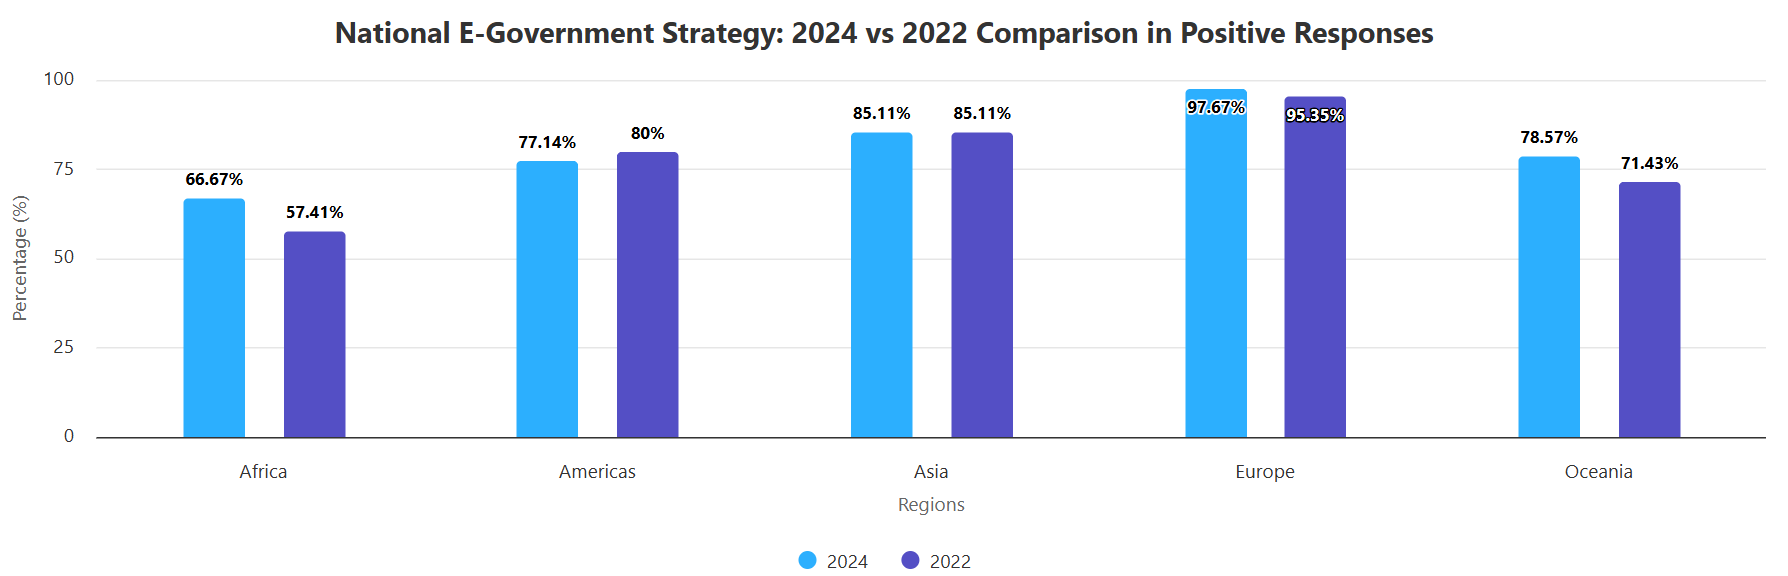
\includegraphics[width=1\linewidth]{figuras/ict_in_government/national_government_strategy}
	\label{fig:national_government_strategy}
	\footnotesize{Fonte: \cite{ONU_ICT_in_government_indicators}}
\end{figure}

\begin{figure}[H]
	\centering
	\caption{Indicador: Existência de identidade digital para acessar ou outra forma de autenticação requirida para poder acessar serviços online}
	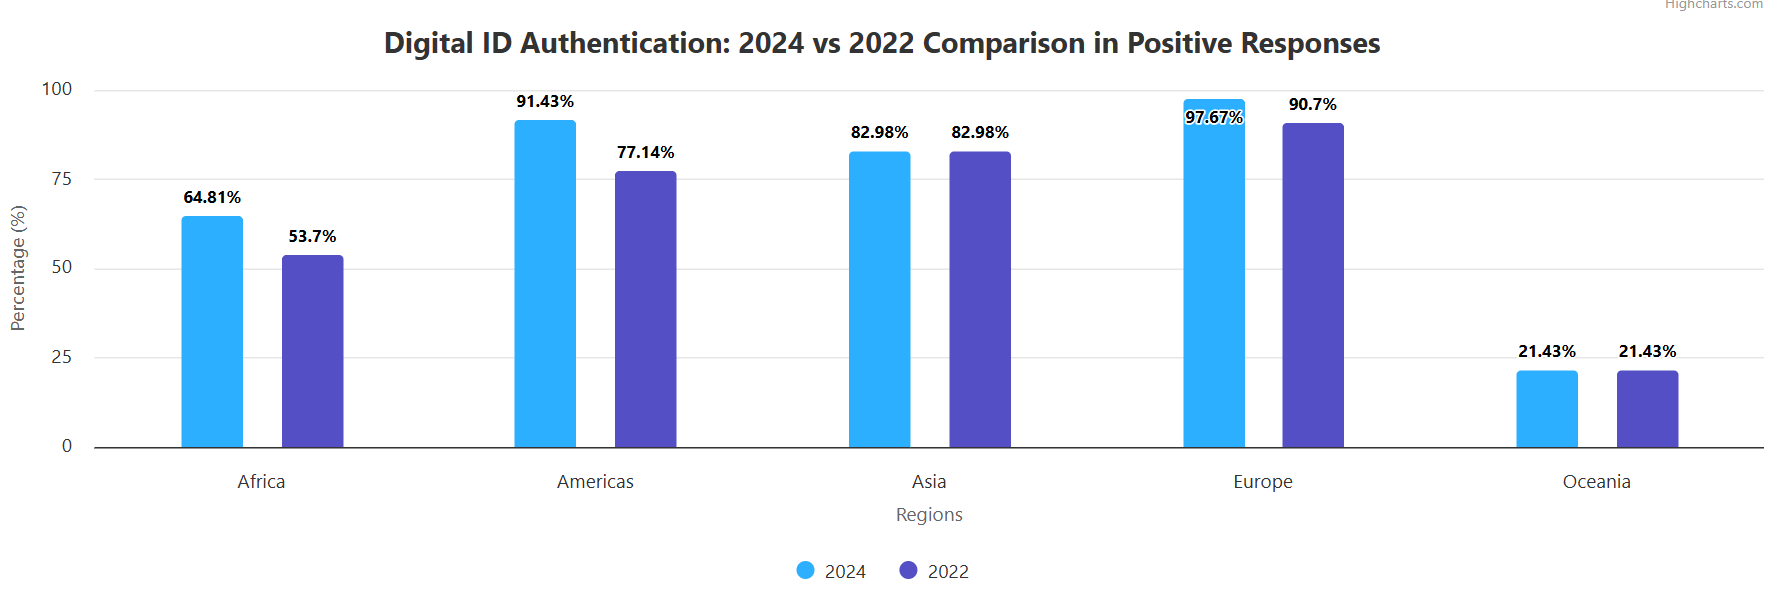
\includegraphics[width=1\linewidth]{figuras/ict_in_government/digital_identity}
	\label{fig:national_identity}
	\footnotesize{Fonte: \cite{ONU_ICT_in_government_indicators}}
\end{figure}

\begin{figure}[H]
	\centering
	\caption{Indicador: Existência de um portal de compras governamentais}
	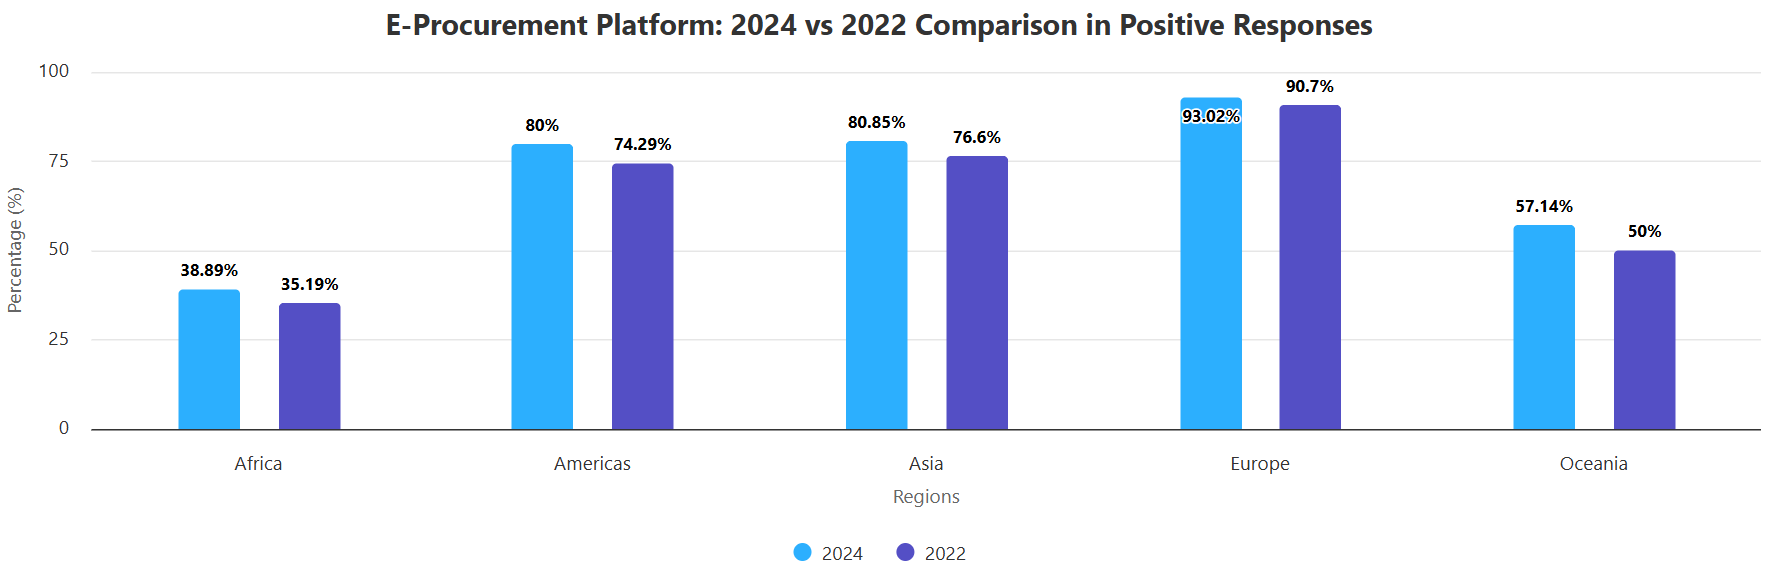
\includegraphics[width=1\linewidth]{figuras/ict_in_government/procurement_portal}
	\label{fig:procurement_portal}
	\footnotesize{Fonte: \cite{ONU_ICT_in_government_indicators}}
\end{figure}

Das três figuras, a Europa foi o continente cujos mais respondem que têm seguem os indicadores, superando os 90\%. A Oceania foi o continente que menos implementou políticas de identidade digital para acesso a serviços online. África e Oceania tiveram um desempenho ruim na implementação de portais de compra governamentais. O continente americano apresentou bom desempenho nos três indicadores.

Como consequência da análise dos resultados presentes nas figuras \ref{fig:national_government_strategy}, \ref{fig:national_identity} e \ref{fig:procurement_portal}, buscou-se entender a seguinte situação registrada nos 2022 e 2024, anos em que os indicadores foram medidos: qual é a porcentagem de países que responderam nenhuma, uma, duas ou todas as perguntas. Elas usam sim ou não para confirmar a aplicação dos indicadores no país.

A resposta ao questionamento está presente na figura \ref{fig:indicators_answer}.

\begin{figure}[H]
	\centering
	\caption{Resposta positiva aos indicadores de TIC de governo eletrônico}
	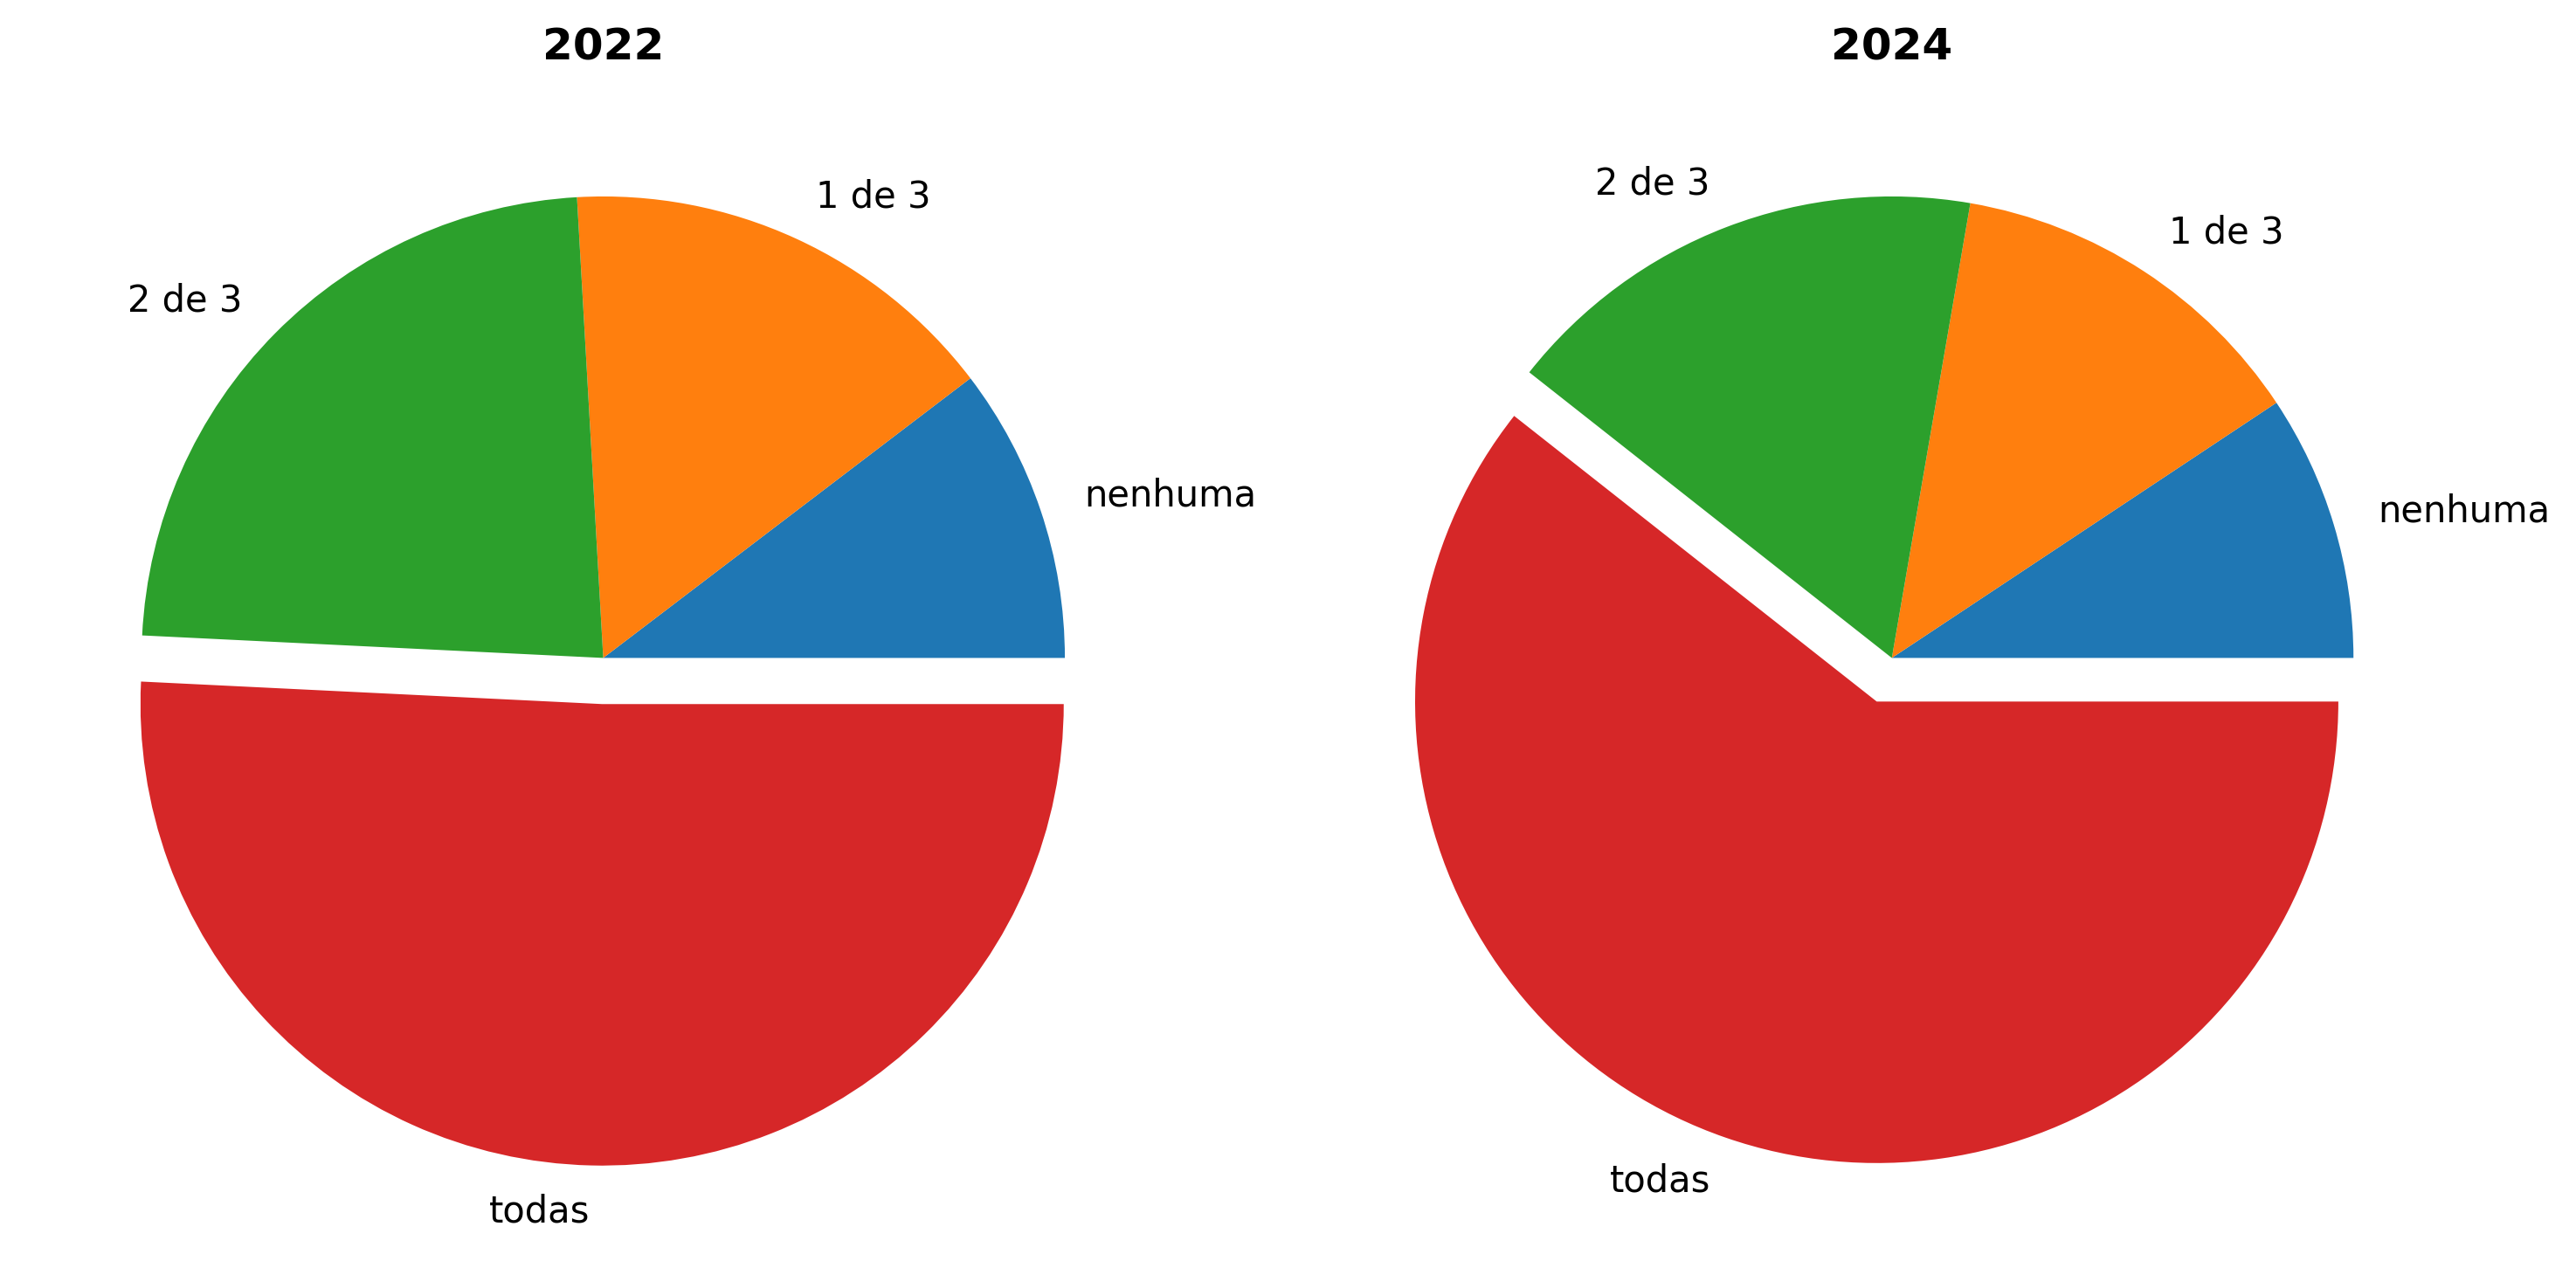
\includegraphics[width=1\linewidth]{figuras/ict_in_government/indicators_answer}
	\label{fig:indicators_answer}
	\footnotesize{Fonte: \cite{ONU_ICT_in_government_indicators}}
\end{figure}

Em 2022, metade dos países respondeu positivamente as três perguntas; em 2024, mais da metade. O Brasil faz parte desse grupo, tal como a Rússia e China. A mudança é creditada a redução do número de países que responderam positivamente 2 de 3 perguntas e passaram a responder as três positivamente. 

Além, disso a quantidade de países que responderam positivamente 1 de 3 perguntas e nenhuma se igualou em 2024, sendo os países que responderam 1 de 3 perguntas era maior do que os que responderam nenhuma.

Tal detalhe se alinha à não correlação entre o EGDI e o índice de democracia eleitoral. Porém, buscou-se entender se há correlação entre os indicadores de TIC de governo eletrônico e o PIB \textit{per capita} PPC.